\documentclass[12pt]{article}
\usepackage[utf8]{inputenc}
\usepackage{amsmath}
\usepackage{graphicx}
\usepackage{hyperref}
\usepackage[spanish]{babel}
\usepackage{parskip}  % Paquete para controlar la sangría y el espaciado entre párrafos
\usepackage{graphicx}  % Paquete para incluir imágenes
\usepackage{tocbibind}  % Para incluir el índice de imágenes en el índice general
\usepackage{amsfonts}
\usepackage{float}

\setlength{\parindent}{1em}  % Establece la sangría de los párrafos
\setlength{\parskip}{0.5em}   % Establece el espaciado entre los párrafos

\title{\Huge Visión Artificial}
\author{\Large Juan Diego Gallego Nicolás\\ \href{mailto:jdiego.gallego@um.es}{jdiego.gallego@um.es}}
\date{\Large 23/03/2025}

\begin{document}

\maketitle
\thispagestyle{empty}

% Portada
\begin{center}
    \vspace{2cm}
    \textbf{Entrega Parcial}
\end{center}

\newpage

% Índice
\tableofcontents
\newpage

% Índice de imágenes
\listoffigures
\newpage

% Sección 1: Introducción
\section{Introducción}
Este documento recoge explicaciones y resultados de los ejercicios realizados durante el desarrollo de la asignatura
siguiendo las instrucciones del repositorio de GitHub albertoruiz/umucv/blob/master/notebooks/ejercicios.ipynb (revisado el 20/03/2025).
Cada ejercicio se corresponde con la sección del documento con el mismo nombre.
A su vez, cada sección se divide en los subapartados: Marco Teórico, Resultados y Comentarios.

La sección Marco Teórico servirá como resumen de los contenidos teóricos desarrollados en la teoría necesarios para la realización de la práctica. 
A continuación, en el apartado de Resultados se hablará del trabajo realizado (código y pruebas) y de cómo se han aplicado los conocimientos teóricos.
Finalmente, la sección Comentarios se reserva para realizar alguna reflexión y plasmar las conclusiones y opiniones sobre el ejercio.

Las imágenes incluidas son capturas de pantalla de Geogebra clásico (www.geogebra.org/classic?lang=es) y Geogebra 3D (www.geogebra.org/3d?lang=es), material de la asignatura, gráficas de matplotlib e imágenes tomadas con un Google Pixel 8 Pro.

A lo largo del documento se hará mención a una serie de scripts de python desarrollados por el profesor Alberto Ruiz. Estos scripts se encuentran en el repositorio de GitHub albertoruiz/umucv/ (revisado el 20/03/2025).

\newpage

% Sección 2: Calibración
\section{Calibración}

\subsection{Calibración: Marco Teórico}

Una cámara es un dispositivo compuesto esencialmente por una lente que enfoca luz en un plano de proyección.
Ese plano de proyección físico se sitúa detraś de la lente y de forma invertida. Tras deshacer la inversión, los dispositivos de visualización presentan la imagen en la orientación correcta.
Nótese que el proceso de reconstrucción de la imagen genera un plano de proyección virtual con las mismas dimensiones y a la misma distancia a la lente que el plano real \ref{fig:Modelo_camara}.

\begin{figure}[h!]
    \centering
    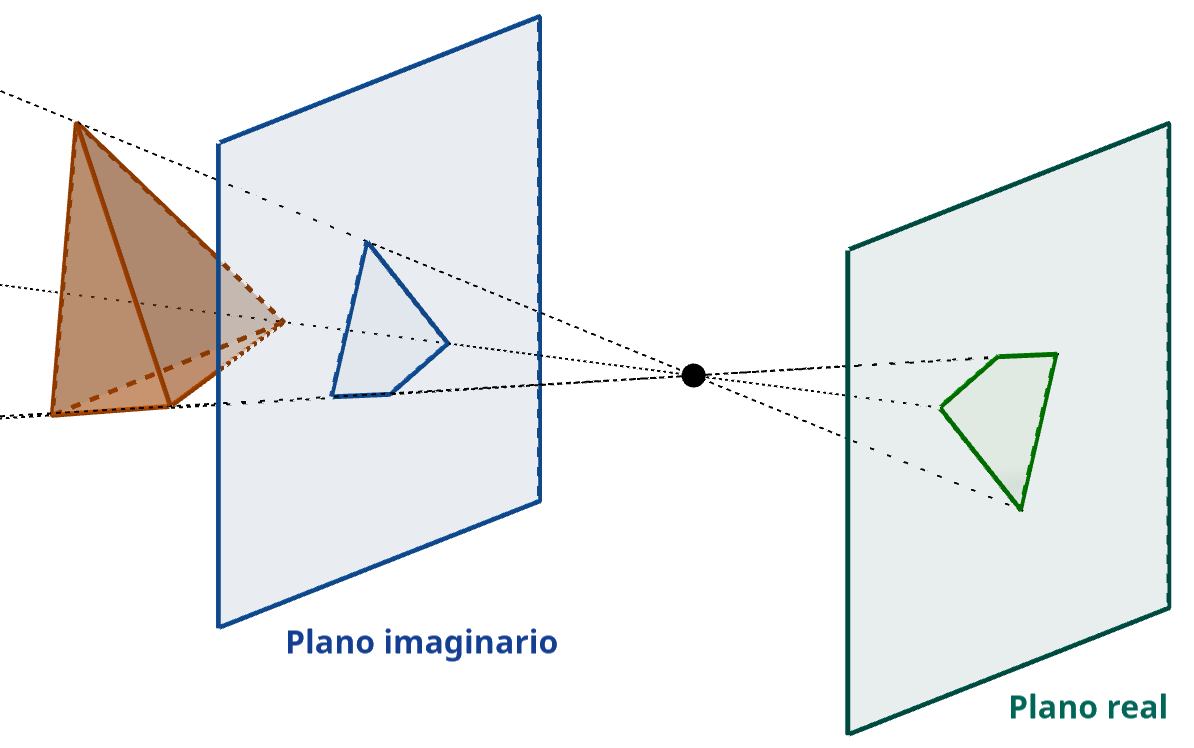
\includegraphics[width=0.7\textwidth]{images_calibracion/Modelo_camara.png}  % Cambia 'imagen_ejemplo.jpg' por el nombre de tu archivo
    \caption{Modelo de una cámara.}
    \label{fig:Modelo_camara}
\end{figure}

Hay dos parámetros esenciales que describen las propiedades de una cámara: su resolución y su distancia focal. 
La resolución hace referencia a las dimensiones del plano de proyección.
Esta se mide en píxeles (unidad mínima de representación de color) y se puede presentar como el par $W \times H$ o como el número de total píxeles en el plano.
La distancia focal es la distancia entre el foco de la lente y el plano de proyección. También se mide en píxeles.

Calibrar la cámara consiste en aproximar lo máximo posible estos parámetros. Una vez conocidos, se pueden hacer mediciones en el mundo real de distancias, dimensiones y ángulos como veremos más adelante. 
En el caso de esta práctica, usaremos un patrón cuadriculado para este proceso \ref{fig:cuadricula}, aprovechando las distorsiones de tamaños y de los ángulos rectos.

\begin{figure}[h!]
    \centering
    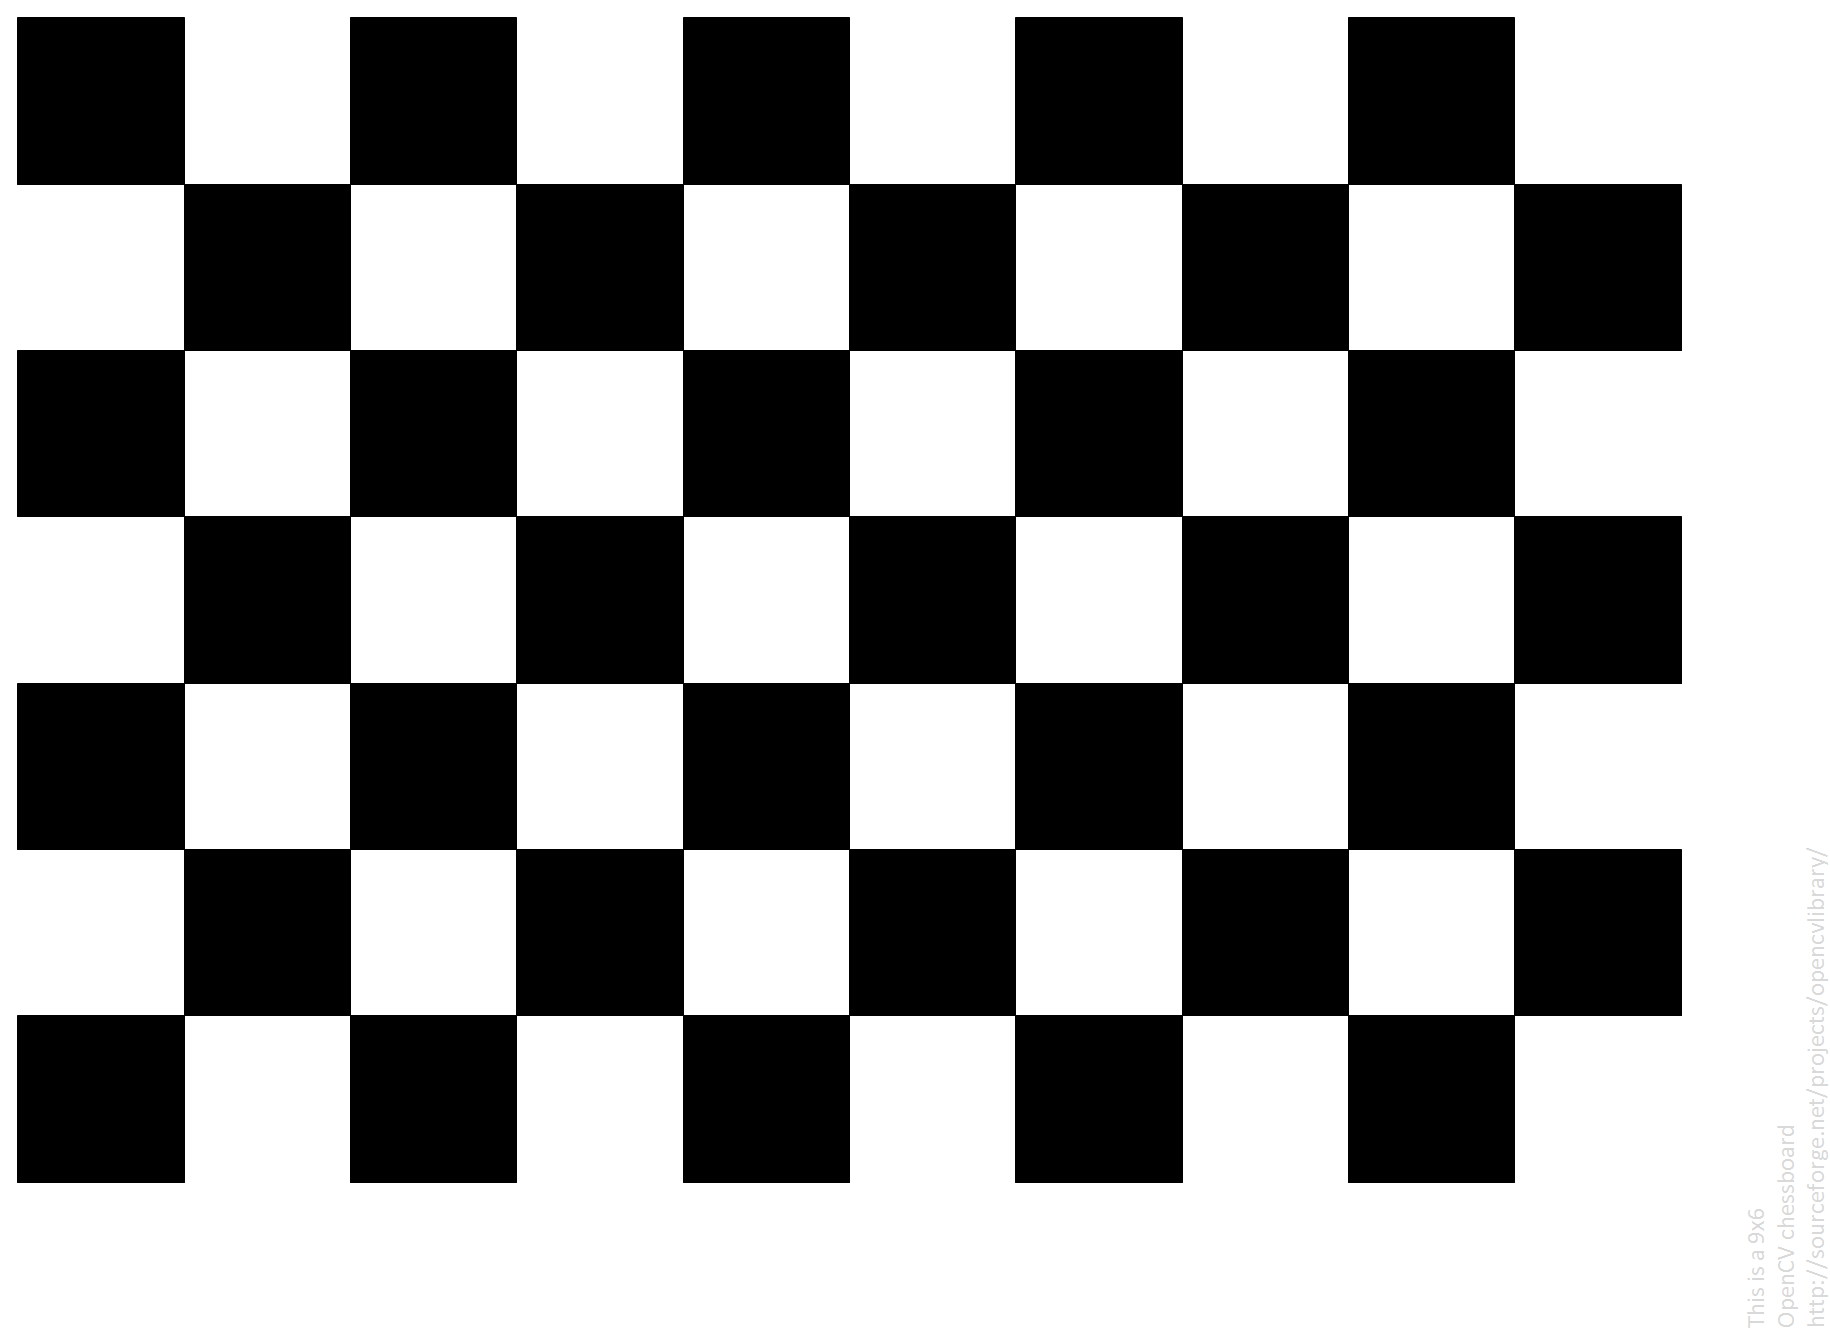
\includegraphics[width=0.7\textwidth]{images_calibracion/Patron_calibracion.png}  % Cambia 'imagen_ejemplo.jpg' por el nombre de tu archivo
    \caption{Patrón para la calibración de la cámara.}
    \label{fig:cuadricula}
\end{figure}

El proceso de calibración da como resultado una matriz $K \in \mathcal{M}_{3 \times 3} (\mathbb{R})$:
$$
K=
\begin{bmatrix}
f & 0 & o_x \\
0 & f_r & o_y \\
0 & 0 & 1
\end{bmatrix}
$$
donde:
\begin{itemize}
    \item[--] $f, f_r$ es la distancia focal y un valor cercano
    \item[--] $(o_x,o_y)$ son las coordenadas en las que se sitúa la proyección del foco de la cámara (normalmente $(W/2,H/2)$)
\end{itemize}

Una propiedad de la cámara interesante, derivada de los parámetros anteriores, es el campo de visión o FOV (Field Of View). 
Es una medida angular que representa las amplitudes horizontal y veltical máximas reconocibles por la cámara \ref{fig:Modelo_fov}.
Aplicando trigonometría básica se derivan las siguientes fórmulas para el FOV horizontal y vertical:
$$ FOV_H = 2*arctan \left( \frac{w}{2f} \right) \text{;     } FOV_V = 2*arctan \left( \frac{h}{2f} \right)$$ 
\begin{figure}[h!]
    \centering
    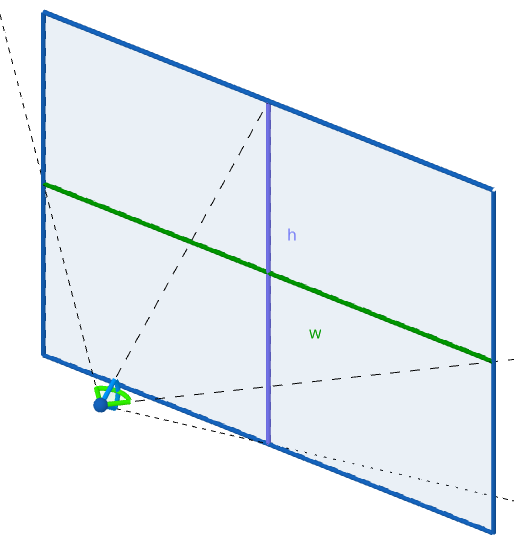
\includegraphics[width=0.7\textwidth]{images_calibracion/Modelo_fov.png}  % Cambia 'imagen_ejemplo.jpg' por el nombre de tu archivo
    \caption{FOV}
    \label{fig:Modelo_fov}
\end{figure}
También, a partir del FOV se deduce la unidad angular mínima medible como $\frac{FOV_H}{W} = \frac{FOV_V}{H}$.

La última propiedad que necesitamos para la realización de la práctica es la relación entre tamaño, tamaño aparente, distancia a la lente y distancia focal.
Esta la podemos obtener aplicando el Teorema de Tales aplicado a los triángulos formados por el foco de la cámara y los pares de extremos reales y virtuales del objeto proyectado \ref{fig:Tales}. 

Claro está que para que esto funcione el objeto a medir ha de estar lo más centrado posible, ya que en los extremos de la imagen se produce distorsión. En las imagenes tomadas para este documento se ha intentado centrar lo máximo posible las imagenes evitando así dicho efecto.

\begin{figure}[H]
    \centering
    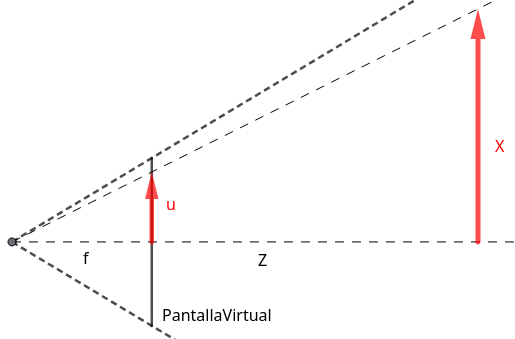
\includegraphics[width=0.6\textwidth]{images_calibracion/Tales.png}  % Cambia 'imagen_ejemplo.jpg' por el nombre de tu archivo
    \caption{Medidas sobre la imagen.}
    \label{fig:Tales}
\end{figure}

\subsection{Calibración: Resultados}

La realización de los ejercicios se puede ver en el notebook de python 'calibracion.ipynb'. 

El primer paso para la realización de la práctica es la calibración de la cámara. 
Para comenzar, he utilizado el programa 'stream.py' para tomar imágenes del patrón \ref{fig:cuadricula} desde una variedad de posiciones y ángulos \ref{fig:calibracion}. 
\begin{figure}[H]
    \centering
    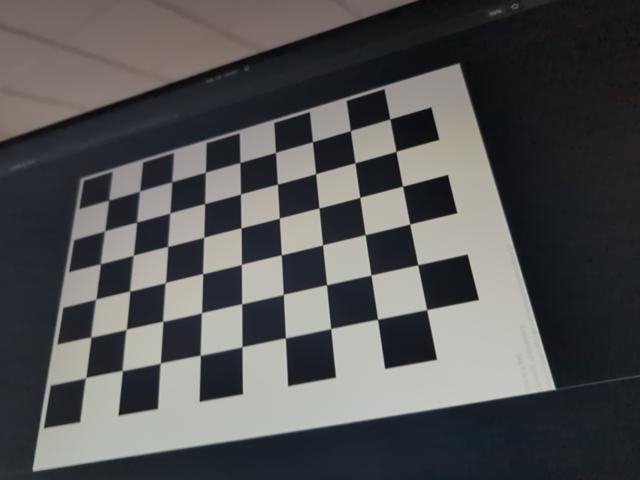
\includegraphics[width=0.6\textwidth]{images_calibracion/Calibracion.png}  % Cambia 'imagen_ejemplo.jpg' por el nombre de tu archivo
    \caption{Fotografía tomada para calibración.}
    \label{fig:calibracion}
\end{figure}
Es importante que exista una variedad en los ángulos de captura ya que la funcionalidad findChessboardCorners de OpenCV utiliza la distorsión en los ángulos de las esquinas de los cuadrados para calcular los parámetros que buscamos.

Una vez tenemos las imágenes, usamos el programa 'calibracion.py' para calibrar la cámara, dando como resultado la matriz de calibración:
$$
K=
\begin{bmatrix}
    561.11 & 0.0000 & 317.80 \\
    0.0000 & 561.09 & 234.53 \\
    0.0000 & 0.0000 & 1.0000
\end{bmatrix}
$$
para una resolución de $640 \times 480$. Con los programas 'triangulate.py' y 'verify.py' podemos comprobar que el proceso se ha completado con éxito.

Con la distancia focal obtenida podemos calcular el $FOV$ de la cámara:
$$FOV_H = 2*arctan \left( \frac{w}{2f} \right) = 59.39^{\circ}$$ 
$$FOV_V = 2*arctan \left( \frac{h}{2f} \right) = 46.32^{\circ}$$
Con este valor, podemos calcular la altura a la que tendríamos que situar la cámara para capturar por completo una pista de baloncesto.
A partir de sus dimensiones ($28 \times 15$ metros):
$$
tan(\frac{FOV_H}{2}) = \frac{28/2}{h_1} \Rightarrow h_1 = \frac{14}{tan(FOV_H/2)}=24.5485625m
$$
$$
tan(\frac{FOV_V}{2}) = \frac{15/2}{h_2} \Rightarrow h_2 = \frac{7.5}{tan(FOV_V/2)}=17.5346875m
$$
De entre los dos resultados tenemos que tomar el mayor, pues necesitamos que la pista se vea tanto a lo largo como a lo ancho.

Buscando el tamaño del resto de líneas de la pista podemos hacer una representación en 3D que nos hace a la idea de la situación que experimentaría la cámara en estas condiciones \ref{fig:pista_basket}:
\begin{figure}[H]
    \centering
    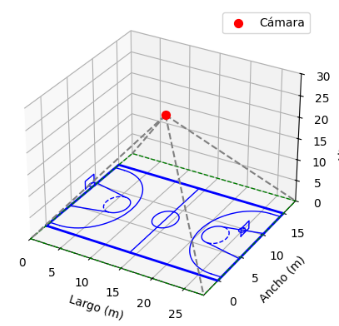
\includegraphics[width=0.6\textwidth]{images_calibracion/Pista_basket.png}  % Cambia 'imagen_ejemplo.jpg' por el nombre de tu archivo
    \caption{Cámara sobre la pista de baloncesto.}
    \label{fig:pista_basket}
\end{figure}
Como se puede observar, sobra espacio mas a allá bandas debido a que la altura necesaria para ver la distancia entre los laterales era menor. 
También se intuye que al estar a una determinada altura las canastas no son entran dentro de la pirámide que constituye el espacio de visión de la cámara.
Aun así, posteriormente supondremos que las canastas se encuentran a nivel de suelo.

Podemos aprovechar el modelo de la pista para simular el tamaño de una pelota de baloncesto situada a diferentes alturas del círculo central \ref{fig:pelota}. 


\newpage

% Sección 3: Filtros
\section{Filtros}
En esta sección se describen los diferentes filtros utilizados en el proceso de procesamiento de imágenes. Los filtros son herramientas esenciales para mejorar la calidad de las imágenes antes de aplicar técnicas de visión artificial más avanzadas.



\newpage

% Sección 4: Clasificador
\section{Clasificador}
Aquí se hablará sobre los clasificadores utilizados para la tarea específica. Se puede incluir la descripción de los algoritmos empleados, su rendimiento y los datos con los que se entrenaron.


% Incluir la imagen
\begin{figure}[h!]
    \centering
    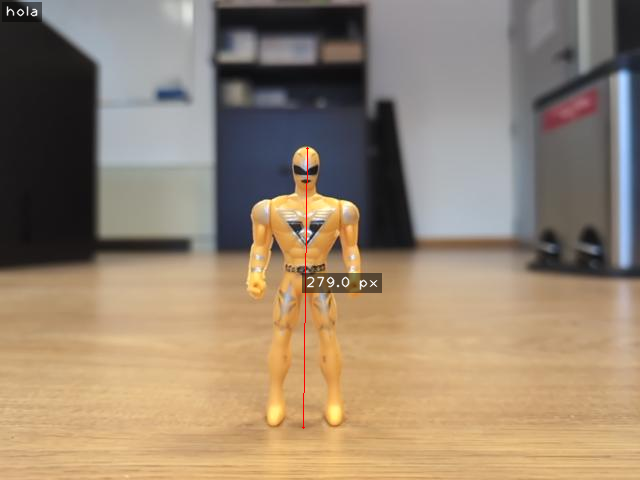
\includegraphics[width=0.7\textwidth]{images_calibracion/Altura_objeto.png}  % Cambia 'imagen_ejemplo.jpg' por el nombre de tu archivo
    \caption{Una imagen de ejemplo.}
    \label{fig:imagen_ejemplo}
\end{figure}

Como se puede ver en la \ref{fig:imagen_ejemplo}, esta es una imagen de ejemplo que se utiliza en el documento.

\end{document}